%!TEX root = ../../Main.tex
\graphicspath{{Chapters/Opgave1/}}
%-------------------------------------------------------------------------------

\chapter{Data Analyse}

\section{Datasæt}
Opgave 1 bygger på et datasæt, der er velagt opgaven. Datasættes indeholder data fra en vejecelle som er belastet med henholdsvis 1 Kg og dernæst 0 Kg. Med andre ord er der et offset i vejedataen. Dataen er samplet med 300 Hz. 

\section{Analyse}
I første del af opgaven skal det udleverede datasæt analyseres. Analysen kommer til at bygge på udregninger af gennemsnit, varians og spredning. Dette gør vi for at kunne fortælle noget om hvor meget dataen varierer, og hvor tæt dataen er fordelt omkring en given middelværdi. For at kunne behandle dataen som loaded og unloaded, altså med og uden belastning, deles signalet i første gang op i to datasæt.

\begin{figure}[H]
\centering
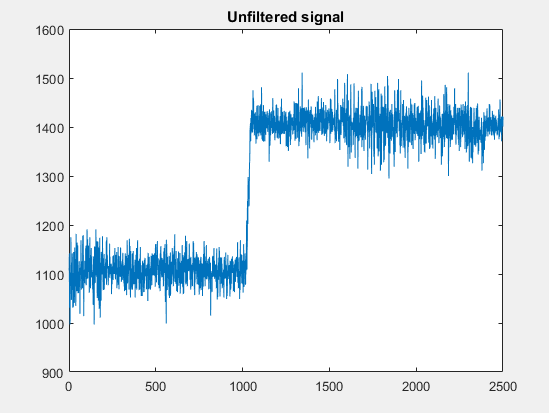
\includegraphics[width = 300pt]{Img/IndenOpdeling.PNG}
\caption{Plottet datasæt inden opdeling}
\label{fig:IndenOpdeling}
\end{figure}

\begin{figure}[H]
\centering
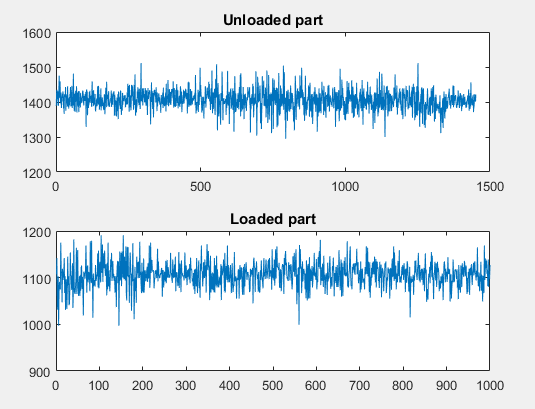
\includegraphics[width = 300pt]{Img/EfterOpdeling.PNG}
\caption{Plottet datasæt efter opdeling}
\label{fig:EfterOpdeling}
\end{figure}

Ud fra de nye to datasæt kan nu beregning en middelværdi. Dette gøres ved at summere alle samples i et datasæt og dele med antal samples herefter. Dette gøres for såvel det loadede datasæt som det unloadede datasæt.

\begin{figure}[H]
\centering
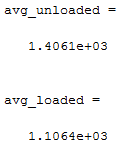
\includegraphics{Img/Middelvaerdi.PNG}
\caption{Middelværdi udregning i matlab for loaded og unloaded datasæt}
\label{fig:Middelvaerdi}
\end{figure}

Herefter kan variansen og spredning for de to datasæt beregnes. For at finde variansen tages et givent samples og trækkes middelværdien fra. Denne sum kvadreres og udføres for hvert enkelt sample i datasættet. Alle disse lægges herefter sammen og deles med n altså antal samples. Nedenstående ses formel for udregning af varians. 

\begin{figure}[H]
\centering
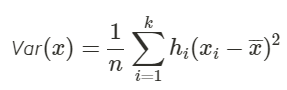
\includegraphics{Img/Varians.PNG}
\caption{Formel for udregning af varians}
\label{fig:Varians}
\end{figure}

Med udgangspunkt i den fundne varians for begge datasæt, kan spredningen findes. Spredningen findes som kvadratroden af variansen. Denne er et udtryk for hvor meget et givent datasæt spreder sig omkring middelværdien. Altså om der er mange datapunkter der ligger langt fra middelværdien eller om disse centrerer sig. Nedenstående ses udregningen af varians og spredning(deviation) for begge vores datasæt.

\begin{figure}[H]
\centering
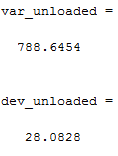
\includegraphics{Img/VariansSpredningUnloaded.PNG}
\caption{Udregning af varians og spredning for det ikke belastede datasæt}
\label{fig:VariansSpredningUnloaded}
\end{figure}

\begin{figure}[H]
\centering
\includegraphics{Img/VariansSpredningloaded.PNG}
\caption{Udregning af varians og spredning for det belastede datasæt}
\label{fig:VariansSpredningloaded}
\end{figure}

Det ses at spredningen på de to datasæt er meget ens. Det vil sige vægtens præcision ikke er synderligt påvirket af hvorvidt denne er belastet eller ej. Med det senere midlingsfilter der ønskes implementeret er det denne spredning vi ønsker at reducere. Dette ønsker vi selvfølgelig i og med vægten gerne skulle måle samme værdi såfremt belastningen er konstant.
\newpage

\section{Visualisering}
For at visualisere vores data plottes histogrammer for begge datasæt. Ud fra disse kan vi gøre os nogle overvejelser omrking hvorvidt vores udregnede spredninger er korrekte. 

\begin{figure}[H]
\centering
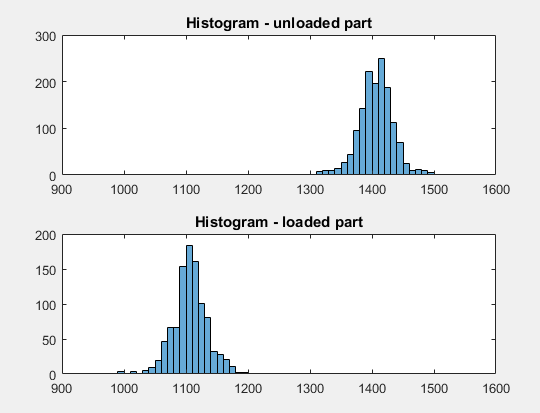
\includegraphics[width = 300pt]{Img/Histogram.PNG}
\caption{Histogram plot for såvel loaded som unloaded datasæt}
\label{fig:Histogram}
\end{figure}

Det ses af historgrammerne af begge datasæt er tilnærmelsesvis normalfordelte. Jævnfør normalfordelingsteori ved vi at 95 procent af et datasæt skal ligge indenfor plus minus 2 gange spredningen. For vores datasæt har vi ikke begge tilfælde en spredning på ca. 28. Derfor kan vi se på histogrammet og se at indenfor plus minus 56 i forhold til middelværdien, skal 95 procent af datasættet ligge. Dette stemmer meget godt overens her.  
\newpage 

\section{Effektspektre}
For at kunne sige noget om den støj der ligger i vores datasæt, altså veje målingerne, ønsker vi at plotte et effektspektrum. Dette gøres for hele signalet, det vil sige både loaded og unloaded. Måden dette gøres på er ved at tage den absolutte værdi af FFT på vores signal. Derefter plotter vi dette kvadreret. Samtidig vælger vi at plotte effektspektret på en DB skala for lettere at kunne overskue signalets niveauer. 

\begin{figure}[H]
\centering
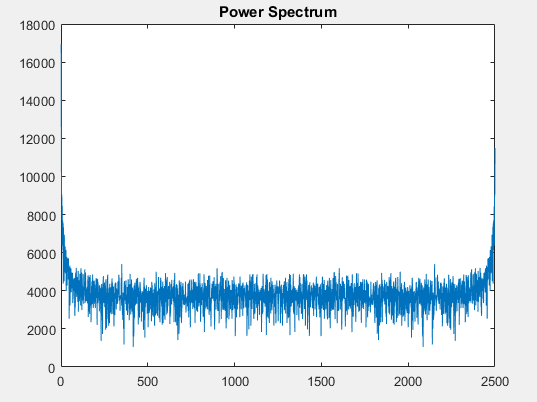
\includegraphics[width = 300pt]{Img/Effekt.PNG}
\caption{Effektspektrum for signalet}
\label{fig:Effekt}
\end{figure}

Det ses at støjen på signalet er meget ligeligt fordelt igennem hele signalet. Vi betragter derfor støjen i signalet som hvid støj. 

\section{Bit-Niveauer}
Som sidste del af analyse fasen ønsker vi at bestemme bitniveauerne i vores datasæt. Altså hvor mange gram et bit vil svarer til (LSB i gram). Dette gøres ved at tage vores middelværdier for loaded og unloaded og trække fra hinanden for derefter at dele med 1000 for at få niveaurne i gram. Dette giver os hvor mange bit et gram svarer til. Vi ønsker dog at vide den modsatte, altså hvor mange gram hvert bit svarer til, hvorfor vi tager det reciprokke heraf. Vi får at bit pr. gram fås til 0.2996 mens gram pr. bit fås til 3.3372. 

